% Template adapted from https://github.com/jgm/pandoc-templates/blob/master/default.latex
% To be used with XeLaTex in memoiR
%%%%%%%%%%%%%%%%%%%%%%%%%%%%%%%%%%%%%%%%%%%%%%%%%%%%%%%%%%%%%%%%%%%%%%%%%%%%%%%%%%%%%%%%%

% Options for packages loaded elsewhere
\PassOptionsToPackage{unicode=true}{hyperref}
\PassOptionsToPackage{hyphens}{url}
\PassOptionsToPackage{dvipsnames,svgnames*,x11names*}{xcolor}
% Right to left support


\documentclass[
  12pt,
  american,
  a4paper,
  extrafontsizes,onecolumn,openright
  ]{memoir}

% Double (or whatever) spacing

% Math
\usepackage{amssymb, amsmath}
% mathspec: arbitrary math fonts
\usepackage{unicode-math}
\defaultfontfeatures{Scale=MatchLowercase}
\defaultfontfeatures[\rmfamily]{Ligatures=TeX,Scale=1}

% Fonts
\usepackage{lmodern}
\usepackage{fontspec}
% Main font
% Specific sanserif font
% Specific monotype font
% Specific math font
% Chinese, Japanese, Corean fonts

% Use upquote for straight quotes in verbatim environments
\usepackage{upquote}
% Use microtype
\usepackage[]{microtype}
\UseMicrotypeSet[protrusion]{basicmath} % disable protrusion for tt fonts

% Verbatim in note

% Color links
\usepackage{xcolor}

% Strikeout

% Necessary for code chunks
\usepackage{color}
\usepackage{fancyvrb}
\newcommand{\VerbBar}{|}
\newcommand{\VERB}{\Verb[commandchars=\\\{\}]}
\DefineVerbatimEnvironment{Highlighting}{Verbatim}{commandchars=\\\{\}}
% Add ',fontsize=\small' for more characters per line
\usepackage{framed}
\definecolor{shadecolor}{RGB}{248,248,248}
\newenvironment{Shaded}{\begin{snugshade}}{\end{snugshade}}
\newcommand{\AlertTok}[1]{\textcolor[rgb]{0.94,0.16,0.16}{#1}}
\newcommand{\AnnotationTok}[1]{\textcolor[rgb]{0.56,0.35,0.01}{\textbf{\textit{#1}}}}
\newcommand{\AttributeTok}[1]{\textcolor[rgb]{0.77,0.63,0.00}{#1}}
\newcommand{\BaseNTok}[1]{\textcolor[rgb]{0.00,0.00,0.81}{#1}}
\newcommand{\BuiltInTok}[1]{#1}
\newcommand{\CharTok}[1]{\textcolor[rgb]{0.31,0.60,0.02}{#1}}
\newcommand{\CommentTok}[1]{\textcolor[rgb]{0.56,0.35,0.01}{\textit{#1}}}
\newcommand{\CommentVarTok}[1]{\textcolor[rgb]{0.56,0.35,0.01}{\textbf{\textit{#1}}}}
\newcommand{\ConstantTok}[1]{\textcolor[rgb]{0.00,0.00,0.00}{#1}}
\newcommand{\ControlFlowTok}[1]{\textcolor[rgb]{0.13,0.29,0.53}{\textbf{#1}}}
\newcommand{\DataTypeTok}[1]{\textcolor[rgb]{0.13,0.29,0.53}{#1}}
\newcommand{\DecValTok}[1]{\textcolor[rgb]{0.00,0.00,0.81}{#1}}
\newcommand{\DocumentationTok}[1]{\textcolor[rgb]{0.56,0.35,0.01}{\textbf{\textit{#1}}}}
\newcommand{\ErrorTok}[1]{\textcolor[rgb]{0.64,0.00,0.00}{\textbf{#1}}}
\newcommand{\ExtensionTok}[1]{#1}
\newcommand{\FloatTok}[1]{\textcolor[rgb]{0.00,0.00,0.81}{#1}}
\newcommand{\FunctionTok}[1]{\textcolor[rgb]{0.00,0.00,0.00}{#1}}
\newcommand{\ImportTok}[1]{#1}
\newcommand{\InformationTok}[1]{\textcolor[rgb]{0.56,0.35,0.01}{\textbf{\textit{#1}}}}
\newcommand{\KeywordTok}[1]{\textcolor[rgb]{0.13,0.29,0.53}{\textbf{#1}}}
\newcommand{\NormalTok}[1]{#1}
\newcommand{\OperatorTok}[1]{\textcolor[rgb]{0.81,0.36,0.00}{\textbf{#1}}}
\newcommand{\OtherTok}[1]{\textcolor[rgb]{0.56,0.35,0.01}{#1}}
\newcommand{\PreprocessorTok}[1]{\textcolor[rgb]{0.56,0.35,0.01}{\textit{#1}}}
\newcommand{\RegionMarkerTok}[1]{#1}
\newcommand{\SpecialCharTok}[1]{\textcolor[rgb]{0.00,0.00,0.00}{#1}}
\newcommand{\SpecialStringTok}[1]{\textcolor[rgb]{0.31,0.60,0.02}{#1}}
\newcommand{\StringTok}[1]{\textcolor[rgb]{0.31,0.60,0.02}{#1}}
\newcommand{\VariableTok}[1]{\textcolor[rgb]{0.00,0.00,0.00}{#1}}
\newcommand{\VerbatimStringTok}[1]{\textcolor[rgb]{0.31,0.60,0.02}{#1}}
\newcommand{\WarningTok}[1]{\textcolor[rgb]{0.56,0.35,0.01}{\textbf{\textit{#1}}}}

% Listings package

% Tables
\usepackage{longtable,booktabs,tabu}
% Fix footnotes in tables (requires footnote package)
\IfFileExists{footnote.sty}{\usepackage{footnote}\makesavenoteenv{longtable}}{}

% Graphics
\usepackage{graphicx,grffile}
\graphicspath{{images/}}
\makeatletter
\def\maxwidth{\ifdim\Gin@nat@width>\linewidth\linewidth\else\Gin@nat@width\fi}
\def\maxheight{\ifdim\Gin@nat@height>\textheight\textheight\else\Gin@nat@height\fi}
\makeatother
% Scale images if necessary, so that they will not overflow the page
% margins by default, and it is still possible to overwrite the defaults
% using explicit options in \includegraphics[width, height, ...]{}
\setkeys{Gin}{width=\maxwidth,height=\maxheight,keepaspectratio}

% Prevent overfull lines
\setlength{\emergencystretch}{3em}  
\providecommand{\tightlist}{%
  \setlength{\itemsep}{0pt}\setlength{\parskip}{0pt}}

% Number sections for memoir (secnumdepth counter is ignored)
\setsecnumdepth{section}

% Set default figure placement to htbp
\makeatletter
\def\fps@figure{htbp}
\makeatother

% Spacing in lists
\usepackage{enumitem}

% Polyglossia
\usepackage{polyglossia}
\setmainlanguage{en-US}
\setotherlanguage{fr-FR}
\setotherlanguage{it}

% BibLaTeX
\usepackage[backend=biber,style=authoryear-ibid,isbn=false,backref=true,giveninits=true,uniquename=init,maxcitenames=2,maxbibnames=150,sorting=nyt,sortcites=false]{biblatex}
\addbibresource{references.bib}

% cslreferences environment required by pandoc > 2.7



%%%%%%%%%%%%%%%%%%%%%%%%%%%%%%%%%%%%%%%%%%%%%%%%%%%%%%%%%%
% memoiR format

% Chapter Summary environment 
\usepackage[tikz]{bclogo}
\newenvironment{Summary}
  {\begin{bclogo}[logo=\bctrombone, noborder=true, couleur=lightgray!50]{In a Nutshell}\parindent0pt}
  {\end{bclogo}}
% Syntax:
%
%```{block, type='Summary'}
% Deliver message here.
% ```

% scriptsize code 
\let\oldverbatim\verbatim
\def\verbatim{\oldverbatim\scriptsize}
% Applies to code blocks and R code results
% code chunk options size='scriptsize' applies only to R code and results
% if the code chunk sets a different size, \def\verbatim{...} is prioritary for code results 


% Layout
%%%%%%%%%%%%%%%%%%%%%%%%%%%%%%%%%%%%%%%%%%%%%%%%%%%%%%%%%%

% Based on memoir, style companion
\newcommand{\MemoirChapStyle}{daleif1}
\newcommand{\MemoirPageStyle}{Ruled}

% Space between paragraphs
\usepackage{parskip}
  \abnormalparskip{3pt}

% Adjust margin paragraphs vertical position
\usepackage{marginfix}


% Margins
%%%%%%%%%%%%%%%%%%%%%%%%%%%%%%%%%%%%%%%

% allow use of '-',+','/' ans '*' to make simple length computation
\usepackage{calc}

% Full-width figures utilities
\newlength\widthw % full width
\newlength{\rf}
\newcommand*{\definesHSpace}{
  \strictpagecheck % slower but efficient detection of odd/even pages
  \checkoddpage
  \ifoddpage
  \setlength{\rf}{0mm}
  \else
  \setlength{\rf}{\marginparsep+\marginparwidth}
  \fi
}

\makeatletter
% 1" margins for the front matter.
\newcommand*{\SmallMargins}{
  \setlrmarginsandblock{1.5in}{1.5in}{*}
  \setmarginnotes{0.1in}{0.1in}{0.1in}
 \setulmarginsandblock{1.5in}{1in}{*}
  \checkandfixthelayout
  \ch@ngetext
  \clearpage
  \setlength{\widthw}{\textwidth+\marginparsep+\marginparwidth}
  \footnotesatfoot
  \chapterstyle{\MemoirChapStyle}  % Chapter and page styles must be recalled
  \pagestyle{\MemoirPageStyle}
}

% 3" outer margin for the main matter
\newcommand{\LargeMargins}{\SmallMargins}
\makeatother

% Figure captions and footnotes in outer margins


% Main title page with filigrane
%%%%%%%%%%%%%%%%%%%%%%%%%%%%%%%%%%%%%%%%%%%%%%%%%%%%%%%%%%

% Text blocks
\usepackage[absolute,overlay]{textpos}
  \setlength{\TPHorizModule}{1mm}
  \setlength{\TPVertModule}{1mm}

\newcommand{\MainTitlePage}[2]{
  \SmallMargins % Margins
  \pagestyle{empty} % No header/footer
  \textblockorigin{\stockwidth-\paperwidth-\trimedge}{\trimtop} % recto
  \begin{textblock*}{2mm}(\spinemargin/2,\uppermargin/2)
    \rule{1pt}{\paperheight-\uppermargin}
  \end{textblock*}
  \begin{textblock*}{\paperwidth*2/3}(\paperwidth/5, \paperheight/5)
    \flushright
    \begin{Spacing}{3}
      {\fontfamily{qtm}\selectfont\fontsize{45}{45}\selectfont\textsc{\thetitle}}
    \end{Spacing}
  \end{textblock*}
    \begin{textblock*}{\paperwidth*2/3}(\paperwidth/5, \paperheight/2)
    \flushright
    {\fontfamily{qtm}\huge\theauthor}
  \end{textblock*}
    \begin{textblock*}{\paperwidth*2/3}[0, 1](\spinemargin, \uppermargin+\textheight)
    \normalfont\thedate
  \end{textblock*}
  ~\\ % Print a character or the page will not exist
  \newpage
  \textblockorigin{\trimedge}{\trimtop} % verso
  \begin{textblock*}{\textwidth}(\paperwidth-\spinemargin-\textwidth, \uppermargin)
    #1
  \end{textblock*}
  \begin{textblock*}{\textwidth}[0,1](\paperwidth-\spinemargin-\textwidth, \uppermargin+\textheight+\footskip)
    \centering
    
\includegraphics[width=\paperwidth/4]{logo}\\ \bigskip
    #2
  \end{textblock*}
  ~\\ % Print a character or the page will not exist
  \newpage
}

% Clear page and open an even one (\clearpage opens an odd one)
\newcommand{\evenpage}{
  \clearpage
  \strictpagecheck % slower but efficient detection of odd/even pages
  \checkoddpage
  \ifoddpage
    \thispagestyle{empty}
    ~\\ % Print a character or the page will not exist
    \newpage
  \else
    % do nothing
  \fi
}


%% PDF title page to insert
%%%%%%%%%%%%%%%%%%%%%%%%%%%%%%%%%%%%%%%%%%%%%%%%%%%%%%%%%%

\usepackage{pdfpages}


%% Bibliography
%%%%%%%%%%%%%%%%%%%%%%%%%%%%%%%%%%%%%%%%%%%%%%%%%%%%%%%%%%

\usepackage[strict,autostyle]{csquotes}
% Repeated citation as author-year-title instead of author-title (modification of footcite:note in verbose-inote.cbx)

%% Table of Contents
%%%%%%%%%%%%%%%%%%%%%%%%%%%%%%%%%%%%%%%%%%%%%%%%%%%%%%%%%%

% fix the typesetting of the part number
\renewcommand\partnumberlinebox[2]{#2\ ---\ }


% Fonts
%%%%%%%%%%%%%%%%%%%%%%%%%%%%%%%%%%%%%%%%%%%%%%%%%%%%%%%%%%


% Hyperref comes last
%%%%%%%%%%%%%%%%%%%%%%%%%%%%%%%%%%%%%%%%%%%%%%%%%%%%%%%%%%

\usepackage{hyperref}
\hypersetup{
  pdftitle={User's guide for Ecofog's Ecophysiology Lab},
  pdfauthor={Marion Boisseaux, Daniela Krebber, Tristan Lafont Rapnouil},
  colorlinks=true,
  linkcolor=Maroon,
  citecolor=Blue,
  urlcolor=Blue,
  breaklinks=true}

% Don't use monospace font for urls
\urlstyle{same}


% Title, author, date from YAML to LaTeX
%%%%%%%%%%%%%%%%%%%%%%%%%%%%%%%%%%%%%%%%%%%%%%%%%%%%%%%%%%

\title{User's guide for Ecofog's Ecophysiology Lab}

\author{Marion Boisseaux, Daniela Krebber, Tristan Lafont Rapnouil}

\date{2021-10-31}


% Include headers (preamble.tex) here
%%%%%%%%%%%%%%%%%%%%%%%%%%%%%%%%%%%%%%%%%%%%%%%%%%%%%%%%%%
% Add LaTeX code into the preamble of the document here
\hyphenation{bio-di-ver-si-ty sap-lings}


%%%%%%%%%%%%%%%%%%%%%%%%%%%%%%%%%%%%%%%%%%%%%%%%%%%%%%%%%%%%%%%%%%%%%%%%%
% memoiR dalef3 chapter style 
% https://ctan.crest.fr/tex-archive/info/latex-samples/MemoirChapStyles/MemoirChapStyles.pdf
\usepackage{soul}
\definecolor{nicered}{rgb}{.647,.129,.149}
\makeatletter
\newlength\dlf@normtxtw
\setlength\dlf@normtxtw{\textwidth}
\def\myhelvetfont{\def\sfdefault{mdput}}
\newsavebox{\feline@chapter}
\newcommand\feline@chapter@marker[1][4cm]{%
  \sbox\feline@chapter{%
    \resizebox{!}{#1}{\fboxsep=1pt%
	  \colorbox{nicered}{\color{white}\bfseries\sffamily\thechapter}%
	}}%
  \rotatebox{90}{%
    \resizebox{%
	  \heightof{\usebox{\feline@chapter}}+\depthof{\usebox{\feline@chapter}}}%
	{!}{\scshape\so\@chapapp}}\quad%
  \raisebox{\depthof{\usebox{\feline@chapter}}}{\usebox{\feline@chapter}}%
 }
\newcommand\feline@chm[1][4cm]{%
  \sbox\feline@chapter{\feline@chapter@marker[#1]}%
  \makebox[0pt][l]{% aka \rlap
    \makebox[1cm][r]{\usebox\feline@chapter}%
  }}
\makechapterstyle{daleif1}{
  \renewcommand\chapnamefont{\normalfont\Large\scshape\raggedleft\so}
  \renewcommand\chaptitlefont{\normalfont\huge\bfseries\scshape\color{nicered}}
  \renewcommand\chapternamenum{}
  \renewcommand\printchaptername{}
  \renewcommand\printchapternum{\null\hfill\feline@chm[2.5cm]\par}
  \renewcommand\afterchapternum{\par\vskip\midchapskip}
  \renewcommand\printchaptertitle[1]{\chaptitlefont\raggedleft ##1\par}
}
\makeatother
\usepackage{booktabs}
\usepackage{longtable}
\usepackage{array}
\usepackage{multirow}
\usepackage{wrapfig}
\usepackage{float}
\usepackage{colortbl}
\usepackage{pdflscape}
\usepackage{tabu}
\usepackage{threeparttable}
\usepackage{threeparttablex}
\usepackage[normalem]{ulem}
\usepackage{makecell}
\usepackage{xcolor}


% End of preamble
%%%%%%%%%%%%%%%%%%%%%%%%%%%%%%%%%%%%%%%%%%%%%%%%%%%%%%%%%%


\begin{document}
\frontmatter

% Title page
%%%%%%%%%%%%%%%%%%%%%%%%%%%%%%%%%%%%%%%%%%%%%%%%%%%%%%%%%%

\includepdf[pages=1]{images/mariono.pdf}
\cleardoublepage

\MainTitlePage{This document is reproducible thanks to:

\begin{itemize}
  \item \LaTeX and its class memoir (\url{http://www.ctan.org/pkg/memoir}).
  \item R (\url{http://www.r-project.org/}) and RStudio (\url{http://www.rstudio.com/})
  \item bookdown (\url{http://bookdown.org/}) and memoiR (\url{https://ericmarcon.github.io/memoiR/})
\end{itemize}}{Name of the owner of the logo

\url{http://www.company.com}

An explanatory sentence.
Leave an empty line for line breaks.}


% Before Body
%%%%%%%%%%%%%%%%%%%%%%%%%%%%%%%%%%%%%%%%%%%%%%%%%%%%%%%%%%




% Contents
%%%%%%%%%%%%%%%%%%%%%%%%%%%%%%%%%%%%%%%%%%%%%%%%%%%%%%%%%%

\LargeMargins
{
\hypersetup{linkcolor=}
\setcounter{tocdepth}{2}
\tableofcontents
}


% Body
%%%%%%%%%%%%%%%%%%%%%%%%%%%%%%%%%%%%%%%%%%%%%%%%%%%%%%%%%%

\LargeMargins
\hypertarget{introduction}{%
\chapter*{Introduction}\label{introduction}}
\addcontentsline{toc}{chapter}{Introduction}

This document allows you to create a book in PDF format (and ePub format) at the same time as an HTML version to be published on the web.
The syntax is that of \textbf{Markdown} with some extensions.

The \textbf{bookdown} package must be installed from CRAN or GitHub:

\scriptsize

\begin{Shaded}
\begin{Highlighting}[]
\KeywordTok{install.packages}\NormalTok{(}\StringTok{"bookdown"}\NormalTok{)}
\CommentTok{# or the development version}
\CommentTok{# devtools::install_github('rstudio/bookdown')}
\end{Highlighting}
\end{Shaded}

\normalsize

The book is organized in chapters.
Each chapter is an Rmd file, whose name normally begins with its number (e.g.~\texttt{01-intro.Rmd}).
All Rmd files in the project folder are actually treated as chapters, sorted by filename.
The index.Rmd file is special: it contains the document header and the first chapter.

This first chapter is placed in the foreword of the printed book: it should not be numbered (hence the \texttt{\{-\}} code next to the title) in the HTML version.
It must end with the LaTeX command \texttt{\textbackslash{}mainmatter} which marks the beginning of the body of the book.

The outline levels start with \texttt{\#} for chapters (only one per file), \texttt{\#\#} for sections, etc.

Compilation in PDF format is done by XeLaTeX, which must be installed.

While writing, it is strongly advised to create only the HTML file, which is much faster than a LaTeX compilation.
Each chapter can be viewed very quickly by clicking on the \emph{Knit} button above the source window.
The entire book is created by clicking on the \emph{Build Book} button in the RStudio \emph{Build} window.
The button's drop-down list allows you to create all documents or limit yourself to one format.

\mainmatter

\hypertarget{intro}{%
\chapter{Introduction}\label{intro}}

Plant functional traits are the features (morphological, physiological, phenological) that represent ecological strategies and determine \emph{describe?} how plants respond to environmental factors, affect other trophic levels and influence ecosystem properties. Variation in plant functional traits, and trait syndromes, has proven useful for tackling many important ecological questions at a range of scales, giving rise to a demand for standardized ways to measure ecologically meaningful plant traits. The importance of these topics dictates the urgent need for more and better data, and increases the value of standardized protocols for quantifying trait variation of different species, in particular for traits with power to predict plant- and ecosystem-level processes, and for traits that can be measured relatively easily (Pérez-Harguindeguy et al., 2013)

This handbook presents the different protocols used in the ecophysio lab. We therefore suggest the methodological principles for a more open and transparent science. This handbook not only includes updated methods for the trait measurements, but also includes the excel worksheets for data collection and the associated R-scripts to upload/clean the raw data.

\hypertarget{handbook-architecture}{%
\chapter{Handbook architecture}\label{handbook-architecture}}

This handbook is written for operational ends. As such, it is not a review or scientific paper thoroughly presenting each traits but rather a list of protocols associated with routinely measured traits in this lab.

Each chapter of this book correspond to one trait and associated measurement process.

\hypertarget{morpho-anatomy}{%
\section{Morpho-anatomy}\label{morpho-anatomy}}

\hypertarget{hydraulics}{%
\section{Hydraulics}\label{hydraulics}}

\hypertarget{fluorescence}{%
\section{Fluorescence}\label{fluorescence}}

\hypertarget{fluxes-and-gaz-exchange}{%
\section{Fluxes and gaz exchange}\label{fluxes-and-gaz-exchange}}

\hypertarget{microbial}{%
\section{Microbial}\label{microbial}}

\hypertarget{greenhouse-setups-and-tips}{%
\section{Greenhouse setups and tips}\label{greenhouse-setups-and-tips}}

\hypertarget{machine-info}{%
\section{Machine info}\label{machine-info}}

\hypertarget{root-morphology}{%
\section{Root Morphology}\label{root-morphology}}

Root morphology analysis (length, diameter, etc.) are conducted using the Winrhizo software.

Winrhizo is a licenced software created by Regent Instrument Canada Inc.~It exist 4 different version and we own the \emph{Basic Version}. It allows root morphology analysis from scans.

\hypertarget{image-acquisition}{%
\subsection{Image Acquisition}\label{image-acquisition}}

\hypertarget{format}{%
\subsubsection{Format}\label{format}}

Supported image format are \texttt{.TIFF}, \texttt{.JPEG} and \texttt{.BMP}. \texttt{.TIFF}and \texttt{.BMP} are not compressed and are thus to be preferred. \texttt{.TIFF} images are compatible with all OS and should be privileged but you must be careful to save them \emph{uncompressed} as \texttt{WinRhizo} won't be able to open \emph{compressed} ones.

The higher the resolution, the more pixel you will have and the more precise will be your measurements. However, with resolution, scan time and image size increase. 800DPI is the standard in this lab but 400 is the winrhizo recommendation. This depend on the required level of precision as well as the size of the analyzed roots ( the finer the higher must be the resolution to get more details).

\hypertarget{scanner}{%
\subsubsection{Scanner}\label{scanner}}

Any scanner can be used to acquire scans for Winrhizo software. However, be sure that the format is compatible and that all the images inside your project are saved in the same format and the same resolution. For coherence purposes we encourage you to use the same formats between studies at Ecofog's lab scale.
\href{document/machine/EPSON_V800/test.txt}{EPSON's V800} scanners are the ones used as this document is being written. The scanner model isn't important but we recommend to use scanners with a transparent (double-lamp) option. This will allow cleaner root scans for complex root systems.
And the scanning software is \href{document/software/Viewscan/test.txt}{ViewScan}

\hypertarget{scan-process}{%
\subsubsection{Scan process}\label{scan-process}}

Paste the wall-taped doc.

\hypertarget{flat-scan}{%
\paragraph{Flat scan}\label{flat-scan}}

You can decide to use basic scan options with light only coming from below. If you do so you need to have a white background installed under the scanner's roof (if black roots, if pale ones you'll need a black background).

Choosing this option will simplify your protocol and can suffice for simple and thin enough root systems.

\textbf{EXEMPLE} scan marion

\hypertarget{transparent}{%
\paragraph{Transparent}\label{transparent}}

If your root are too big \ref{fig:bigroots}, then self-shading can appear on flat scan and bias winrhizo's analysis. To avoid this shading you can remove the background from the scanner's roof to enable double-lamp scanning. The light coming from top and bottom as one, shading will be avoid and scans will be cleaner.

\scriptsize

\begin{figure}

{\centering 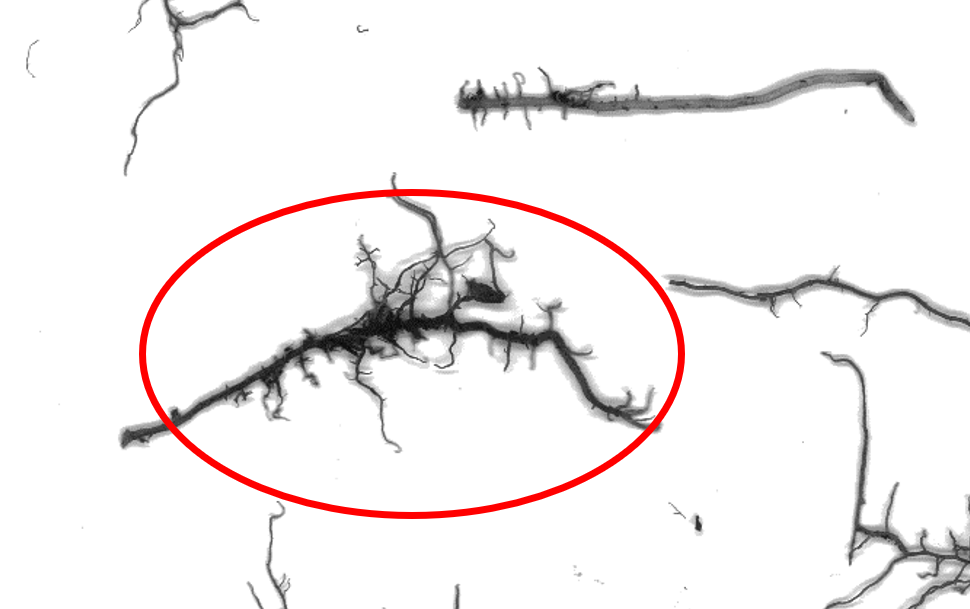
\includegraphics[width=0.5\linewidth]{document/trait/rootmorpho/thickroot} 

}

\caption{Roots to thick to be flat scanned}\label{fig:bigroots}
\end{figure}

\normalsize

Another case where you can prefer \texttt{Transparent} option is for complex root systems (e.g.~bromeliaceae, \ref{fig:bromeroot}) . For this type of roots, you can scan them in a thin coat of water to disentangle fine roots. Doing so you will have a better analysis of the root system morphology and structure but once again have shading issue. Supressing them requires the use of the \texttt{Transparent} mode.

\scriptsize

\begin{figure}

{\centering 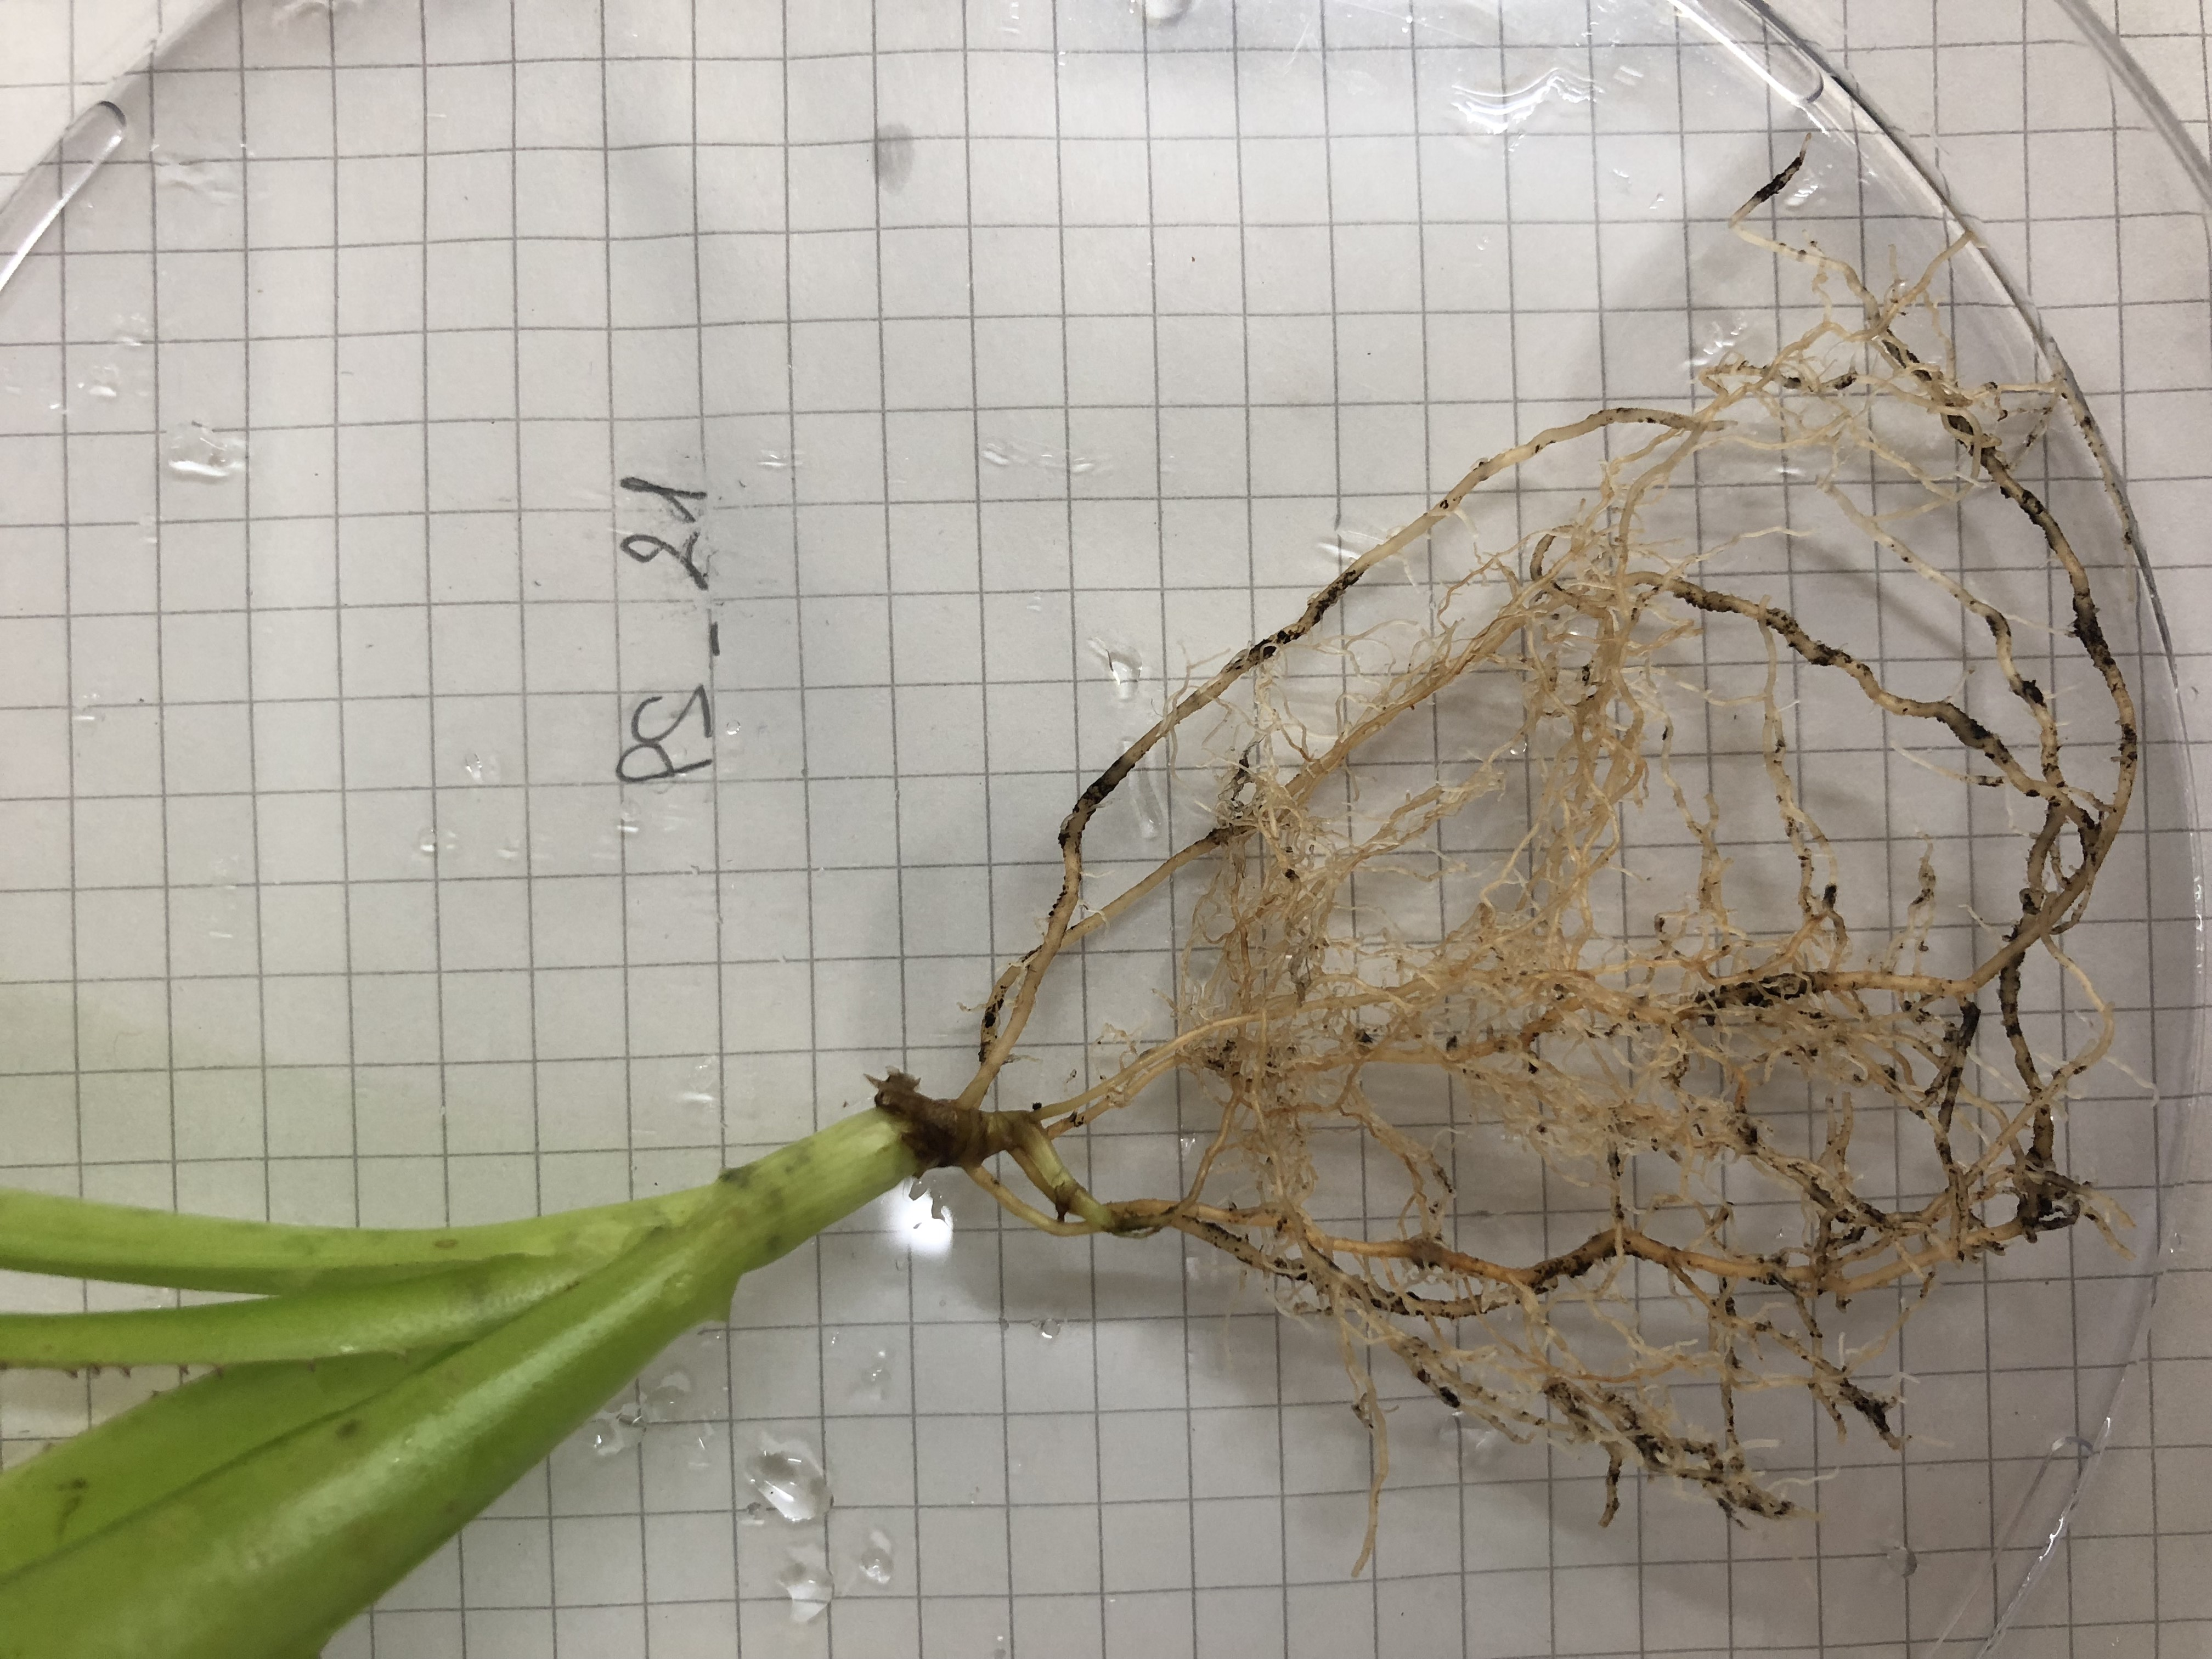
\includegraphics[width=0.5\linewidth]{document/trait/rootmorpho/bromeroot} 

}

\caption{Complex bromeliad adventitious root system}\label{fig:bromeroot}
\end{figure}

\normalsize

\textbf{BEWARE:} The \texttt{Transparent} scan window is smaller than the normal mode scan. The actual scanned zone is showed \ref{fig:scantransp} and you must make sure that you roots are well placed within this area.

\scriptsize

\begin{figure}

{\centering 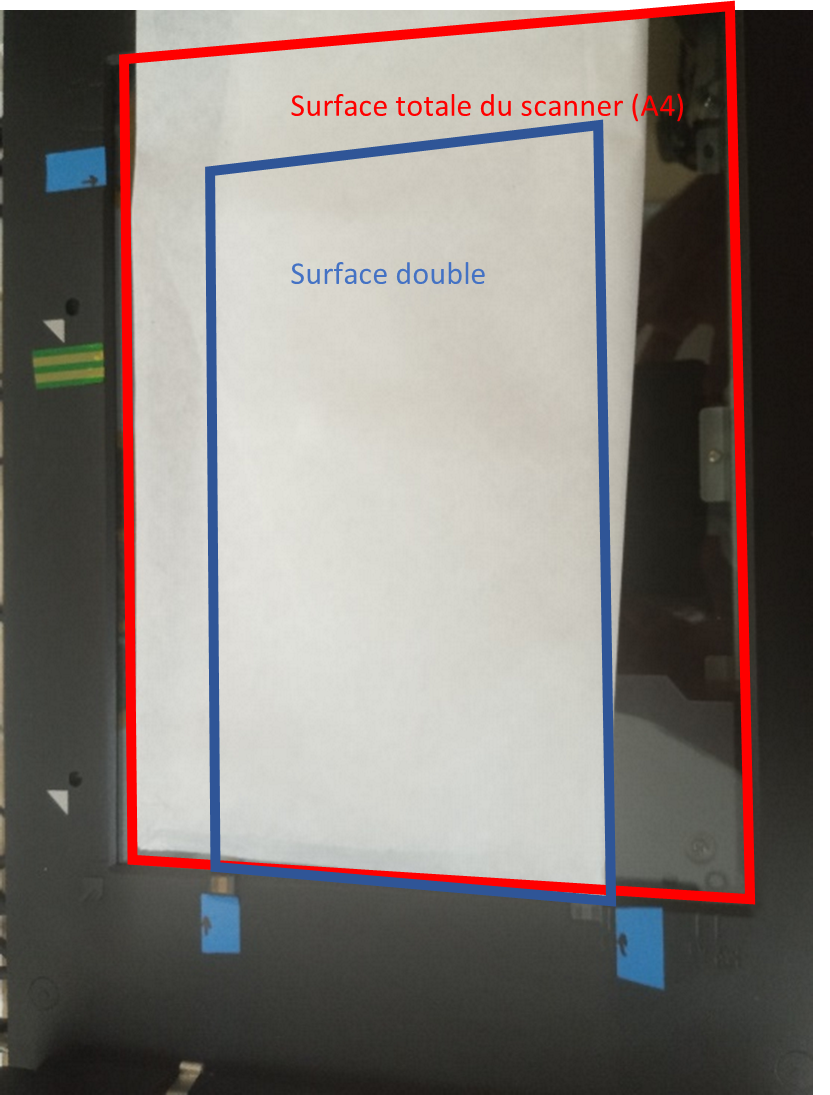
\includegraphics[width=0.5\linewidth]{document/trait/rootmorpho/scan_transp} 

}

\caption{Flat (red) and Transparent (blue) scan zone of EPSON's V800 scanner}\label{fig:scantransp}
\end{figure}

\normalsize

\hypertarget{image-processing}{%
\subsection{Image processing}\label{image-processing}}

To analyze with winrhizo, you can either make it manually, one image at a time and by drawing rectangles around the roots you want to analyze.
However, when having a lot of scans you might want to automatize the process using the \texttt{batch} option.
If this is your choice, make sure that your images only contain roots!! Sometimes you will have to remove some parts of the scans to leave only roots in your images.
For instance, this \ref{fig:bromescan} is the scan from bromeliads roots. We can see the water-filled petri dishes border on the scan and this will be an issue for automatized Winrhizo analysis.

\scriptsize

\begin{figure}

{\centering 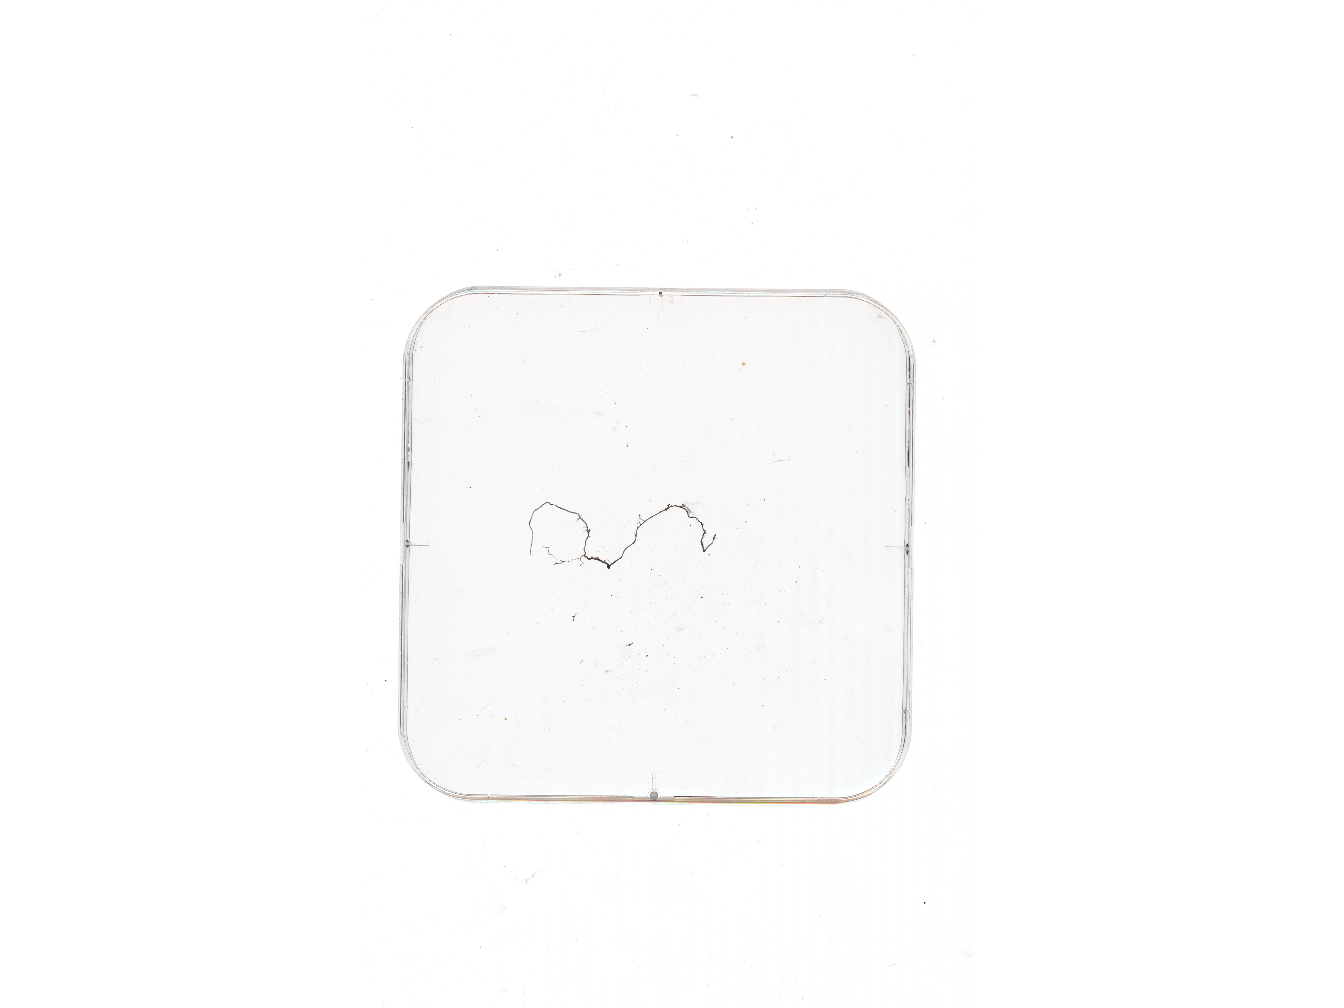
\includegraphics[width=0.5\linewidth]{MyBook_files/figure-latex/bromescan-1} 

}

\caption{Scan of a bromeliad root system in water-filled petri dish}\label{fig:bromescan}
\end{figure}

\normalsize

To re-crop these images we use the freeware \texttt{XnConvert}. The petri dish has always been placed in the same place using a stencil \ref{fig:scanstencil} on the scan window, enabling us to recrop all scans to the same size.
Detailed \texttt{XnConvert} tutorial is available \href{document/software/XnConvert/test.txt}{HERE}.

\scriptsize

\begin{figure}

{\centering 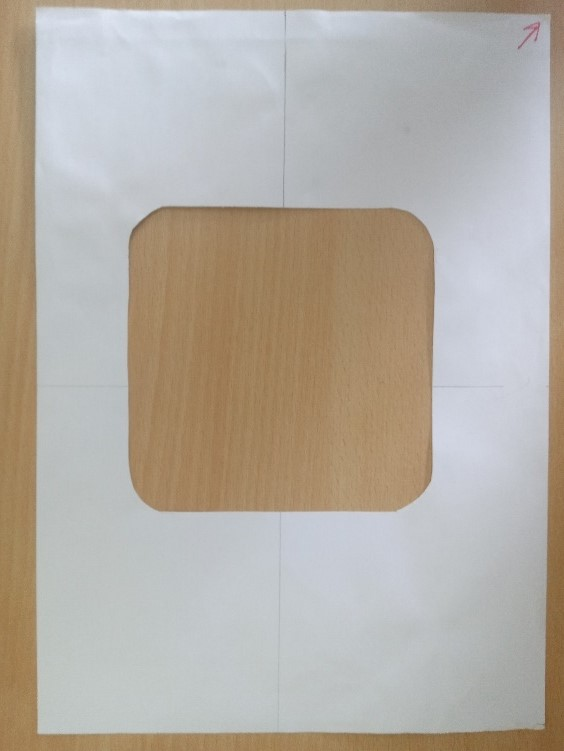
\includegraphics[width=0.5\linewidth]{document/trait/rootmorpho/squre_stencil} 

}

\caption{Stencil used for inwater root scans}\label{fig:stencil-1}
\end{figure}
\begin{figure}

{\centering 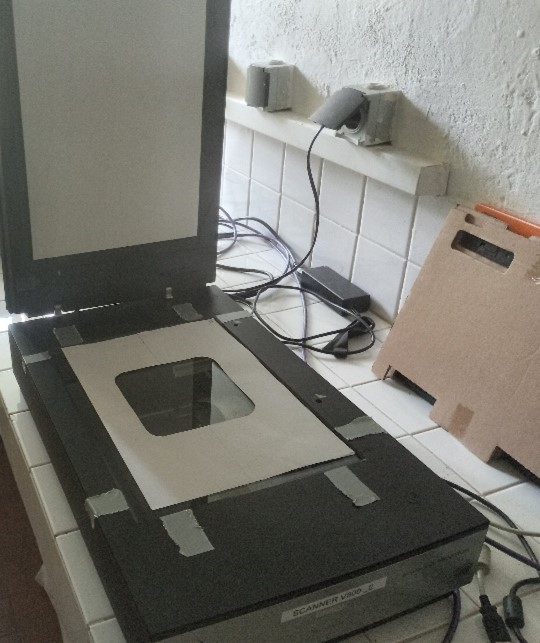
\includegraphics[width=0.5\linewidth]{document/trait/rootmorpho/squre_stencil2} 

}

\caption{Stencil used for inwater root scans}\label{fig:stencil-2}
\end{figure}

\normalsize

\hypertarget{winrhizo}{%
\subsection{WinRhizo}\label{winrhizo}}

\hypertarget{installation}{%
\subsubsection{Installation}\label{installation}}

The winrhizo software is contained on a CD (ask \href{https://docs.google.com/spreadsheets/d/1EqjCVr6w7fykUJtLOVwSNBucNfFGbiYXGlRcoL-s7V8/edit\#gid=0}{\textbf{Eliane Louisanna}}. To be used you need to copy the software from the disk to your computer and install the protection key drivers (also on the CD). Once installed you don't need the CD to run the software but the protection key must be plugged. Unplugging it will prevent any use of the software.

\hypertarget{startup}{%
\subsubsection{Startup}\label{startup}}

\hypertarget{first-analysis}{%
\subsubsection{First analysis}\label{first-analysis}}

Once you have acquired your images and launched winrhizo you can start to analyze your scans. To display a single scan, click \emph{Image} -\textgreater{} \emph{Origin} -\textgreater{} \emph{From File}. Then you can click the \emph{acquisition }icon \textbf{PIC}.
This will open a standard document opening window. Then you browse normally to find the wanted scan. Make sure that you are looking for the goor format, by default, winrhizo display \texttt{.TIFF}.
When you open it, winrhizo display the targeted image and you can then click on it (analyze whole image) or make a selection (only selected region) to start an analysis.

When an image or region is analyzed, winrhizo display the \emph{sample identification} window which allows you to enter information about the sample. These informations will be saved with the measurements data. In this window click \emph{OK} to do the analysis or \emph{Cancel} to abort it.

After you clicked \emph{OK}, winrhizo starts the analysis (can be stopped pressing \emph{S}). When done, winrhizo is ready to save the data but a file must be opened or created first.
Winrhizo display a window which asks wether to \emph{open one}, \emph{create one} or \emph{save nothing}. Selecting \emph{create one} will create a new \texttt{.TXT} file to store analysis data (more info about output \protect\hyperlink{output}{here}). Selecting \emph{open one} will allow you to open a pre-existing file to add the new measurements at the end of this file. Clicking on \emph{save nothing}, guess?

In the image, you can now see which roots have been analyzed. This have a skeleton line over them. The absence of this skeleton indicates that these roots have not been analyzed. This can be due to non-optimal pixel classification (see more about it \protect\hyperlink{pixel-classification}{here}).

WELL DONE! You just analyze your first picture!

You can practice with scans available \protect\hyperlink{resources}{here}

\hypertarget{calibration}{%
\subsubsection{Calibration}\label{calibration}}

If not calibrated (associated with a scale), winrhizo will display results in pixels. \texttt{.TIFF} files have an embedded scale, automatically detected by winrhizo. Check on your results if they are in px (pixels), in (inches) or cm (centimeters).

However, you can sometimes have uncalibrated files (mistakes or images from camera). Thus, you will need to \enquote{manually} calibrate your image. Winrhizo calibration files are saved as \texttt{.CAL}. In the \emph{Calibration} menu you can load pre-existing calibration files. You will find the \texttt{calib\_imge.TIFF} \href{document/trait/rootmorpho/calib_imge.TIF}{here}. To make your calibration at any DPI, you can print this image and scan it at the wanted DPI. The black square in the image delimit a white 1x1cm square. Loading this image in winrhizo, you can click on \emph{calibration} -\textgreater{} \emph{pixel size method} -\textgreater{} \emph{object of known dimension} -\textgreater{} \emph{1 image} -\textgreater{} width=1 , height=1, border=0.35, units=cm -\textgreater{} \emph{Ok}

Then, winrhizo will propose you to save the calibration in a \texttt{.CAL} file that can be loaded later and used for all your images at a given resolution. \textcolor{red}{DO NOT NAME YOUR FILE Scanner.cal}.
Please, when you create a \texttt{.CAL} at a previously not used resolution, store a copy of the calibration file \href{document/software/Winrhizo/}{here} so that your work helps your successors!!

\hypertarget{batch}{%
\subsubsection{Batch}\label{batch}}

We saw how to analyze a \protect\hyperlink{first-analysis}{single picture or region}but you might have numerous scans to analyze and want to automatize this process. To do so you will give winrhizo a \emph{batch} (i.e.~a folder) containing any number of images you want.

\hypertarget{pixel-classification}{%
\subsubsection{Pixel classification}\label{pixel-classification}}

\hypertarget{output}{%
\subsubsection{Output}\label{output}}

\hypertarget{resources}{%
\section{Resources}\label{resources}}

\hypertarget{leaf-turgor-loss-point-pi_tlp}{%
\subsection{\texorpdfstring{Leaf turgor loss point, \(\pi_{tlp}\)}{Leaf turgor loss point, \textbackslash pi\_\{tlp\}}}\label{leaf-turgor-loss-point-pi_tlp}}

We assessed the leaf turgor loss point, \(\pi_{tlp}\) in MPa, from a previously established relationship with the osmotic potential at full hydration, \(\pi_{osm}\) in MPa. \(\pi_{osm}\) is linked to the equilibrium solute concentration value \(C_0\) (in mmol.kg\^{}\{-1\}) directly measured with a vapor pressure osmometer (Vapro 5600, Wescor, Logan, UT). This is referred as the \emph{osmometer method} (Bartlett et al.~2012a; Maréchaux et al.~2016).

\hypertarget{materials}{%
\subsection{Materials}\label{materials}}

\begin{itemize}
\tightlist
\item
  Vapor pressure osmometer (Vapro 5520, Wescor, Logan, UT)
\item
  Vapro software (Vapro Lab Report)
\item
  Fridge
\item
  Liquid Nitrogen
\item
  Ziplock bag\\
\item
  Paper towel
\item
  Distilled water
\item
  Metal tea ball
\item
  Tin foil
\item
  Needle\\
\item
  Liquid nitrogen gloves + goggles
\item
  Liquid nitrogen contenant
\item
  2 Tweezers
\item
  Cork borer
\end{itemize}

\hypertarget{methods}{%
\subsection{Methods}\label{methods}}

\hypertarget{installing-vapro-for-measurements}{%
\subsubsection{Installing Vapro for measurements}\label{installing-vapro-for-measurements}}

\begin{itemize}
\tightlist
\item
  Turn on Vapro the day before for the thermocouple's stability
\item
  Test Water Quality \emph{cf Vapro\_cheatsheet}
\item
  Clean
\item
  Calibration \emph{cf Vapro\_cheatsheet}
\item
  Control tests \emph{cf Vapro\_cheatsheet}
\item
  Verify temperature
\item
  Always have the black diamond at the center of the display
\end{itemize}

Used daily:
* clean beforehand
* select automatic mode (10 runs)

\hypertarget{sampling-on-the-field}{%
\subsubsection{Sampling on the field}\label{sampling-on-the-field}}

\begin{itemize}
\tightlist
\item
  Collect at least 3 healthy mature leaves on branch
\item
  Place them in sample ziplock bag with:

  \begin{itemize}
  \tightlist
  \item
    wet paper towel
  \item
    Exhale in bag to saturate in CO\textsubscript{2}
  \item
    Annotate bag with sample information
  \end{itemize}
\item
  Zip bag and stock in cooler
\end{itemize}

\hypertarget{lab-measurements}{%
\subsubsection{Lab measurements}\label{lab-measurements}}

\hypertarget{field-day}{%
\paragraph{Field day}\label{field-day}}

\begin{itemize}
\tightlist
\item
  Recut branch under water
\item
  Replace in ziplock bag with wet paper towel
\item
  Put 24h in fridge to hydrate overnight
\end{itemize}

\hypertarget{n1-field-day}{%
\paragraph{N+1 Field day}\label{n1-field-day}}

Vapro:

\begin{itemize}
\tightlist
\item
  check distilled water in vapro reservoir
\item
  clean
\item
  select automatic mode (10 runs)
\item
  make sure vapro software is on
\end{itemize}

Sample measurement:

\begin{itemize}
\tightlist
\item
  Sample from a leaf a 5 mm disc with a cork borer: \emph{avoid 1\textsuperscript{st} and 2\textsuperscript{nd} order veins to avoid apoplastic dilution that would lead to less negative osmometer values}
\item
  Wrap disc in tin foil
\item
  Immerse in liquid nitrogen for at least 2 min using metal tea ball
\item
  Puncture 10-15 times with needle
\item
  Place in vapro chamber
\end{itemize}

In total, disc are exposed to air for less than 40 seconds for all the steps.

\begin{itemize}
\item
  Record value C\textsubscript{0} when the difference between consecutive 2-min measurements fell below strictly 5 mmol.kg\textsuperscript{-1} after at least three runs.
\item
  If error! or Nr\_Run \textgreater{} 10 :
\item
  try a 2\textsuperscript{nd} cycle with same leaf
\item
  try a 3\textsuperscript{rd} cycle with another leaf
\item
  otherwise record \emph{NA}
\item
  Beware of the stuck leaf inside the vapro! If so \emph{cf Vapro\_cheatsheet}
\end{itemize}

\hypertarget{end-measurements}{%
\paragraph{End measurements}\label{end-measurements}}

Clean Vapro

For more information on the vapro machine, please refer to the \emph{vapro cheatsheet} in the machine category.

\hypertarget{leaf-midday-water-potential}{%
\section{Leaf midday water potential \$}\label{leaf-midday-water-potential}}

\hypertarget{pressure-chamber-method}{%
\subsection{Pressure chamber method}\label{pressure-chamber-method}}

\hypertarget{psychrometry-method}{%
\subsection{Psychrometry method}\label{psychrometry-method}}

\hypertarget{relative-water-content-rwc}{%
\section{Relative water content RWC (\%)}\label{relative-water-content-rwc}}

\hypertarget{material}{%
\subsection{Material}\label{material}}

\emph{Ziplock bag
}Paper towel
\emph{Distilled water
}Fridge
\emph{Analytical balance
}Sharpie
\emph{cooler
}envelop

\hypertarget{method}{%
\subsection{Method}\label{method}}

Before going on the field:
* write individual code on ziplock bag
* preweight ziplock bag

On the field:
* collect leaf
* clean leaf with clean paper towel
* place leaf in preweighted corresponding ziplock bag
* place bag in cooler for transport to the lab

In the lab:
* weight the closed ziplock with the leaf (\emph{fresh weight})
* delicately take the leaf out of the bag, wrap it in moist paper towel and place the wrap back in the ziplock bag
* place ziplock bag in the fridge during 24 hours
* 24 hours later, take out the leaf and wipe off water excess
* weight re-hydrated leaf (\emph{saturated weight})
* place leaf in envelop for oven-drying during at least 72h
* weight dry leaf (\emph{dry weight})

Calculate RWC (\%):

RWC = \(\frac{(fresh\ weight-dry\ weight)}{(saturated\ weight-dry\ weight)}\) X 100

From Sapes et al 2020 and Barrs \& Weatherley 1962.

\hypertarget{gmin}{%
\section{gmin}\label{gmin}}

\hypertarget{gs}{%
\section{gs}\label{gs}}

\hypertarget{vapor-pressure-osmometer---vapro-5520-cheatsheet}{%
\chapter{Vapor pressure osmometer - Vapro 5520 cheatsheet}\label{vapor-pressure-osmometer---vapro-5520-cheatsheet}}

\begin{itemize}
\tightlist
\item
  \href{./document/machine/Vapro\%205520/Vapro_cheatsheet.pdf}{\textbf{\(\pi_{TLP}\)} vapro cheatsheet}
\end{itemize}

This template is based on \emph{Bookdown} and the \emph{Memoir} LaTeX class to allow writing a book, a report, a PhD thesis, etc. in \emph{R Markdown}.

The main file is \emph{index.Rmd} which contains the description of the book in its header. All other \emph{.Rmd} files in the folder contain a chapter.
The \emph{references.bib} file contains the bibliography.

This file will have to be deleted, as well as \emph{81-getting\_started.Rmd} and \emph{82-syntax.Rmd}: they have to be replaced by the content of the book.

To get started, create a new R project from this folder.
Then open \emph{index.Rmd} and click on the \emph{Build Book} button in the \emph{Build} window of Rstudio.


% Bibliography
%%%%%%%%%%%%%%%%%%%%%%%%%%%%%%%%%%%%%%%%%%%%%%%%%%%%%%%%%%

\backmatter
\SmallMargins

\printbibliography
\onecolumn


% Tables (of tables, of figures)
%%%%%%%%%%%%%%%%%%%%%%%%%%%%%%%%%%%%%%%%%%%%%%%%%%%%%%%%%%


\cleardoublepage
\LargeMargins
\listoffigures


% After-body (LaTeX code inclusion)
%%%%%%%%%%%%%%%%%%%%%%%%%%%%%%%%%%%%%%%%%%%%%%%%%%%%%%%%%%



% Back cover
%%%%%%%%%%%%%%%%%%%%%%%%%%%%%%%%%%%%%%%%%%%%%%%%%%%%%%%%%%%

% Even page, small margins, no running head, no page number.
\evenpage
\SmallMargins
\thispagestyle{empty}

\begin{normalsize}

\begin{description}

\selectlanguage{english}
\item[Abstract]
English abstract, on the last page.

This is the user's guide of EcoFoG's ecophysiology lab
\item[Keywords]
Keyword in English, As a list.
~\\

\end{description}

\end{normalsize}

\vspace*{\fill}
\centering
\includegraphics[width=.3\textwidth]{images/logo}

\end{document}
